%----------------------------------------------------------------------------------------
%	PACKAGES AND OTHER DOCUMENT CONFIGURATIONS
%----------------------------------------------------------------------------------------

\documentclass[12pt]{article}
\usepackage[utf8]{inputenc}
\usepackage[british,UKenglish,USenglish,english,american]{babel}
\usepackage{graphicx}
\usepackage{listings}
\usepackage[T1]{fontenc}
\begin{document}


\newcommand{\HRule}{\rule{\linewidth}{0.5mm}} % Defines a new command for the horizontal lines, change thickness here

\center % Center everything on the page
 
%----------------------------------------------------------------------------------------
%	HEADING SECTIONS
%----------------------------------------------------------------------------------------

\textsc{\LARGE university Jean-Jaur\`{e}s}\\[1.5cm] % Name of your university/college
\textsc{\large Projet Réseau }\\[0.5cm] % Minor heading such as course title


%----------------------------------------------------------------------------------------
%	TITLE SECTION
%----------------------------------------------------------------------------------------

\HRule \\[0.4cm]
{ \huge \bfseries USER MANUAL}\\[0.4cm] % Title of your document
\HRule \\[1.5cm]
 %----------------------------------------------------------------------------------------
%	LOGO SECTION
%----------------------------------------------------------------------------------------


\includegraphics[scale=0.25]{logo.png}\\[1cm] % Include a department/university logo - this will require the graphicx package
 
%----------------------------------------------------------------------------------------

%----------------------------------------------------------------------------------------
%	AUTHOR SECTION
%----------------------------------------------------------------------------------------

\begin{minipage}{0.4\textwidth}
\begin{flushleft} \large
\emph{Authors:}\\
Quentin \textsc{Rouland}\\
Renan \textsc{Husson}
\end{flushleft}
\end{minipage}
~
\begin{minipage}{0.4\textwidth}
\begin{flushright} \large
\emph{To the attention of :} \\
 M.  \textsc{Jacoboni }
\end{flushright}
\end{minipage}\\[4cm]

% If you don't want a supervisor, uncomment the two lines below and remove the section above
%\Large \emph{Author:}\\
%John \textsc{Smith}\\[3cm] % Your name

%----------------------------------------------------------------------------------------
%	DATE SECTION
%----------------------------------------------------------------------------------------

{\large \today}\\[3cm] % Date, change the \today to a set date if you want to be precise




\clearpage
\tableofcontents
\clearpage

\begin{flushleft}
    \section{Client}
The files on the client are in the client file. So we have to move it.

\begin{figure}
    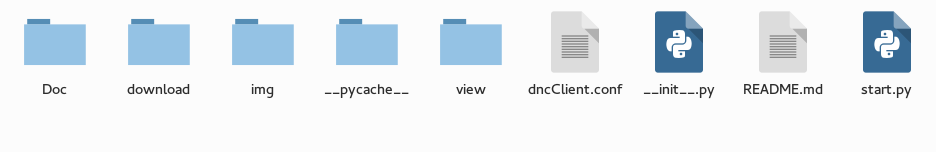
\includegraphics[scale=0.4]{client.png}
    \caption{client folder}
\end{figure}
    
    \subsection{configuration}
Before runing the program, it is possible to change the default configuration file through dncClient.conf. In this file you can configure the port, ip and the nickname. Each client launch, will those parameters will be took into account.

    \subsection{run the client}
The file to run is placed in the client file. Just open a terminal in this folder and run the command
\begin{lstlisting}
 python start.py

 \end{lstlisting} 
  An interface will appear. 
  
  \begin{figure}
    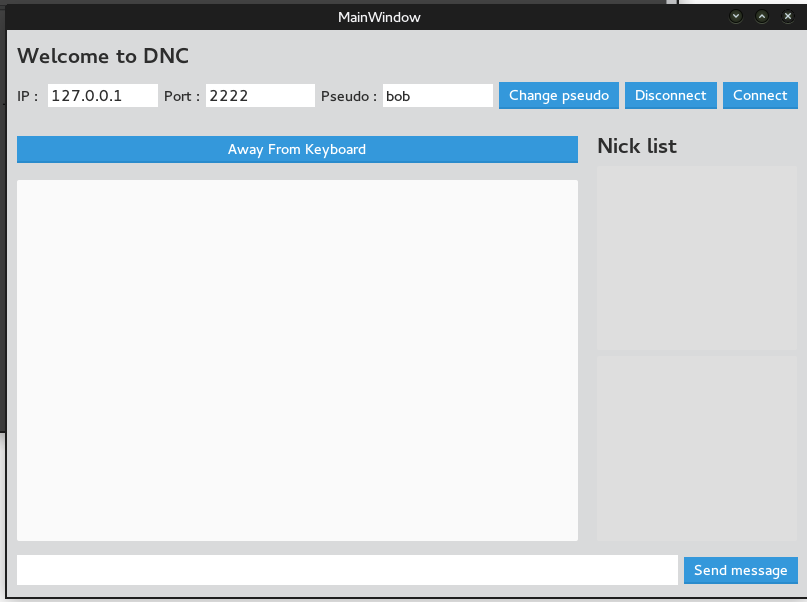
\includegraphics[scale=0.5]{progClient.png}
    \caption{client interface}
\end{figure} 
     
From this interface, it is possible to choose the IP, its port and its nickname. Then just click on Connect. To change your nickname, you must put the new nickname and click nickname changes. To disconnect, simply press disconnect. He wants to have time off and to receive messages during that time, you must press Away from keyboard, and when we come back and we want to again receive messages, just press back.

 \begin{figure}
    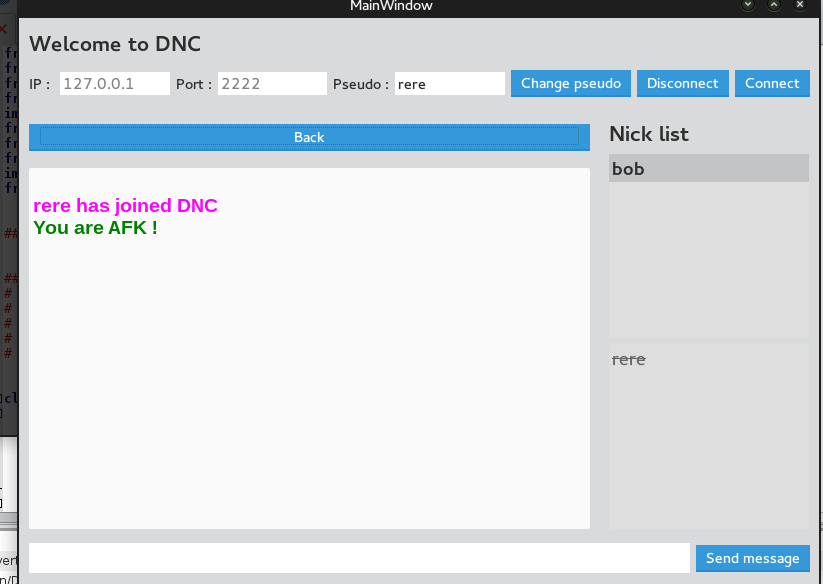
\includegraphics[scale=0.5]{lancement.png}    

    \caption{client interface in action}
\end{figure}
If you wish to make a private conversation with a user, simply right click on his username in the nick list and choose private discussion.If you want to send a file to the user, click on send file.

\begin{figure}
        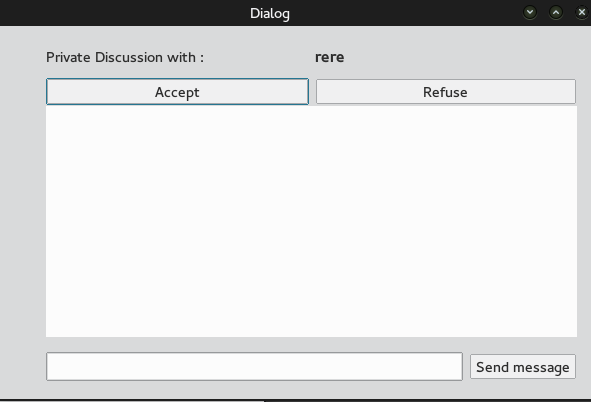
\includegraphics[scale=0.5]{pm.png}
    \caption{private discution}
\end{figure}       
If you receive a private conversation from another user, it is possible to refuse clicking refuses otherwise accept by pressing accept.
    
    \section{Commande}
If you do not wish to use any of the interface buttons, it is of course possible to do everything with just sending command in the text area.

    \subsection{Ask for a private discussion}
Command: /askpm

Parameters: <nickname>

This command ask the client given in parameter for a private chat.


    \subsection{Accept a private discussion}
Command: /acceptpm

Parameters: <nickname>

This command allows the user to start a new conversation with the client given in parameter.
He must receive the /askpm command before.


    \subsection{Reject a private discussion}
Command: /rejectpm
	
Parameters: <nickname>
	
This command finishes or refuses the conversation with the client given in parameter.
He must send the /askpm command before.

    \subsection{Quit}
Command: /quit

Parameters: None

The client ends the connection. It’s used for a clean exit on the server, but it’s also possible to detect when the socket ends.


    \subsection{Private messages}
Command: /pm
Parameters: <nickname> <message>
PRIVMSG is used to send private messages between users. The user must accept the conversation before with /acceptpm.

<nickname> is the nickname of the receiver of the message. <message> is the text to be send to the receiver. <nickname> and <message> cannot be empty.


    \subsection{Disable messages}
    
Command: /disable

Parameters: None

The user stays connected, but don’t receive channel messages and private messages anymore.

    \subsection{Enable messages}
Command: /enable

Parameters: None

This command can only be used after the /disable command. It has the reverse effect.

    \subsection{Change nickname}
Command: /name

Parameters: <nickname>

Allows the user to change his nickname to another. The user must specifies the new nickname in parameter. It must respects the correct format for <nickname>. 


    \subsection{Send a file to an user}
    
    
Command: /pmfile
   
Parameters: <nickname> <file>

The client who wants to send the file sends a request to the file receiver. The request contains the file name and the ip adress of the sender. 
    

    \subsection{Accept file transfert}
Command: /acceptfile 

Parameters: <nickname> <file> <ip> <port>

This command is used in parallel with the rejectfile command to reply to the pmfile command. By using this command, the client will accept receiving a file sended by the client using the pmfile command by the specific port

    \subsection{Reject file transfert}
Command: /rejectfile

Parameters: <nickname> <filename>

This command is used in parallel with the acceptfile command to reply to the pmfile command. By using this command, the client will reject the file sended by the client using the pmfile command.


    \subsection{New nickname}
Command: /newname

Parameters: <nickname>

Allows the user to choose this <nickname> for at connection. 

    \subsection{Get Users Online Connected}
Commande : /userlist

Parameters : None

Request the server to get the userlist connected.


    \subsection{Get Users Away  Connected}
Commande : /userlistaway

Parameters : None

Request the server to get the userlist away.

\clearpage
\listoffigures
\end{flushleft}
\end{document}